\chapter{Renormalization Toolkit}
\section{The Three Key Integrals}
Applying Feynman's rules in Fig.(\ref{fig:loop-integral}), excluding the incoming and outgoing particles, yields the amplitudes under each diagram, where the symbols are defined in (\ref{pi-integral}) to (\ref{lambda-integral})
\begin{figure}[H]
    \centering
\tikzset{every picture/.style={line width=0.75pt}} %set default line width to 0.75pt        

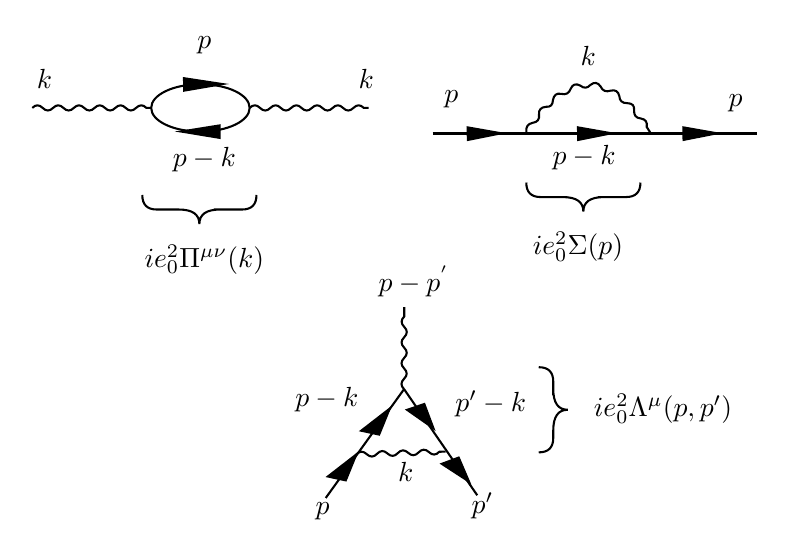
\begin{tikzpicture}[x=0.75pt,y=0.75pt,yscale=-1,xscale=1]
%uncomment if require: \path (0,300); %set diagram left start at 0, and has height of 300

%Straight Lines [id:da8714834249742645] 
\draw    (58.1,71.05) .. controls (59.77,69.38) and (61.43,69.38) .. (63.1,71.05) .. controls (64.77,72.72) and (66.43,72.72) .. (68.1,71.05) .. controls (69.77,69.38) and (71.43,69.38) .. (73.1,71.05) .. controls (74.77,72.72) and (76.43,72.72) .. (78.1,71.05) .. controls (79.77,69.38) and (81.43,69.38) .. (83.1,71.05) .. controls (84.77,72.72) and (86.43,72.72) .. (88.1,71.05) .. controls (89.77,69.38) and (91.43,69.38) .. (93.1,71.05) .. controls (94.77,72.72) and (96.43,72.72) .. (98.1,71.05) .. controls (99.77,69.38) and (101.43,69.38) .. (103.1,71.05) .. controls (104.77,72.72) and (106.43,72.72) .. (108.1,71.05) .. controls (109.77,69.38) and (111.43,69.38) .. (113.1,71.05) -- (115.38,71.05) -- (115.38,71.05) ;
%Shape: Ellipse [id:dp5933813666005416] 
\draw   (115.38,71.05) .. controls (115.38,64.75) and (126,59.64) .. (139.1,59.64) .. controls (152.2,59.64) and (162.82,64.75) .. (162.82,71.05) .. controls (162.82,77.35) and (152.2,82.45) .. (139.1,82.45) .. controls (126,82.45) and (115.38,77.35) .. (115.38,71.05) -- cycle ;
%Straight Lines [id:da5769418846567687] 
\draw    (162.82,71.05) .. controls (164.49,69.38) and (166.15,69.38) .. (167.82,71.05) .. controls (169.49,72.72) and (171.15,72.72) .. (172.82,71.05) .. controls (174.49,69.38) and (176.15,69.38) .. (177.82,71.05) .. controls (179.49,72.72) and (181.15,72.72) .. (182.82,71.05) .. controls (184.49,69.38) and (186.15,69.38) .. (187.82,71.05) .. controls (189.49,72.72) and (191.15,72.72) .. (192.82,71.05) .. controls (194.49,69.38) and (196.15,69.38) .. (197.82,71.05) .. controls (199.49,72.72) and (201.15,72.72) .. (202.82,71.05) .. controls (204.49,69.38) and (206.15,69.38) .. (207.82,71.05) .. controls (209.49,72.72) and (211.15,72.72) .. (212.82,71.05) .. controls (214.49,69.38) and (216.15,69.38) .. (217.82,71.05) -- (220.1,71.05) -- (220.1,71.05) ;
%Shape: Triangle [id:dp6498342909130371] 
\draw  [fill={rgb, 255:red, 0; green, 0; blue, 0 }  ,fill opacity=1 ] (149.68,59.55) -- (131.27,62.72) -- (131.19,56.74) -- cycle ;
%Shape: Triangle [id:dp15479572614043513] 
\draw  [fill={rgb, 255:red, 0; green, 0; blue, 0 }  ,fill opacity=1 ] (129.87,82.43) -- (148.34,79.48) -- (148.32,85.47) -- cycle ;
%Shape: Brace [id:dp8820081102784338] 
\draw   (111.1,113) .. controls (111.1,117.67) and (113.43,120) .. (118.1,120) -- (128.6,120) .. controls (135.27,120) and (138.6,122.33) .. (138.6,127) .. controls (138.6,122.33) and (141.93,120) .. (148.6,120)(145.6,120) -- (159.1,120) .. controls (163.77,120) and (166.1,117.67) .. (166.1,113) ;
%Straight Lines [id:da8146024719775448] 
\draw    (251,83.36) -- (407.18,83.36) ;
%Shape: Triangle [id:dp35521932013796276] 
\draw  [fill={rgb, 255:red, 0; green, 0; blue, 0 }  ,fill opacity=1 ] (337.13,83.27) -- (321.09,86.47) -- (321.02,80.43) -- cycle ;
%Shape: Triangle [id:dp48197684947038777] 
\draw  [fill={rgb, 255:red, 0; green, 0; blue, 0 }  ,fill opacity=1 ] (387.91,83.27) -- (371.87,86.47) -- (371.8,80.43) -- cycle ;
%Shape: Triangle [id:dp4331444823397812] 
\draw  [fill={rgb, 255:red, 0; green, 0; blue, 0 }  ,fill opacity=1 ] (283.99,83.27) -- (267.94,86.47) -- (267.87,80.43) -- cycle ;
%Curve Lines [id:da3147714208948924] 
\draw    (296.17,82.65) .. controls (295.8,80.2) and (296.81,78.72) .. (299.19,78.23) .. controls (301.52,77.9) and (302.54,76.58) .. (302.23,74.29) .. controls (301.99,72) and (303.11,70.74) .. (305.58,70.51) .. controls (307.75,70.7) and (308.87,69.63) .. (308.94,67.31) .. controls (309.37,64.82) and (310.7,63.81) .. (312.93,64.27) .. controls (315.17,64.86) and (316.7,64.03) .. (317.53,61.76) .. controls (318.46,59.64) and (319.99,59.16) .. (322.14,60.31) .. controls (323.9,61.74) and (325.53,61.62) .. (327.04,59.93) .. controls (328.93,58.46) and (330.56,58.73) .. (331.91,60.74) .. controls (332.89,62.85) and (334.5,63.51) .. (336.75,62.73) .. controls (339.06,62.16) and (340.46,63.06) .. (340.95,65.44) .. controls (341.06,67.67) and (342.34,68.77) .. (344.81,68.76) .. controls (347.2,68.81) and (348.28,69.95) .. (348.04,72.18) .. controls (347.91,74.61) and (348.98,75.93) .. (351.25,76.14) .. controls (353.57,76.5) and (354.53,77.86) .. (354.12,80.21) -- (356.4,83.8) ;
%Shape: Brace [id:dp629027508783252] 
\draw   (296.1,107) .. controls (296.1,111.67) and (298.43,114) .. (303.1,114) -- (313.6,114) .. controls (320.27,114) and (323.6,116.33) .. (323.6,121) .. controls (323.6,116.33) and (326.93,114) .. (333.6,114)(330.6,114) -- (344.1,114) .. controls (348.77,114) and (351.1,111.67) .. (351.1,107) ;
%Straight Lines [id:da9660972485295808] 
\draw    (199.48,258.97) -- (237.22,206.54) ;
%Straight Lines [id:da06290426378550174] 
\draw    (237.22,206.54) -- (272.48,257.68) ;
%Shape: Triangle [id:dp7350045088215945] 
\draw  [fill={rgb, 255:red, 0; green, 0; blue, 0 }  ,fill opacity=1 ] (214.21,238.01) -- (209.13,250.5) -- (200.52,248.63) -- cycle ;
%Shape: Triangle [id:dp017358743265808663] 
\draw  [fill={rgb, 255:red, 0; green, 0; blue, 0 }  ,fill opacity=1 ] (230.29,215.94) -- (225.21,228.43) -- (216.59,226.56) -- cycle ;
%Shape: Triangle [id:dp6214973010631918] 
\draw  [fill={rgb, 255:red, 0; green, 0; blue, 0 }  ,fill opacity=1 ] (268.49,251.07) -- (255.4,242.54) -- (263.55,239.51) -- cycle ;
%Straight Lines [id:da4368524173221595] 
\draw    (214.21,238.01) .. controls (215.82,236.29) and (217.49,236.24) .. (219.21,237.85) .. controls (220.93,239.46) and (222.6,239.41) .. (224.21,237.69) .. controls (225.82,235.97) and (227.49,235.92) .. (229.21,237.53) .. controls (230.93,239.14) and (232.59,239.09) .. (234.2,237.37) .. controls (235.81,235.65) and (237.48,235.6) .. (239.2,237.21) .. controls (240.92,238.82) and (242.59,238.76) .. (244.2,237.04) .. controls (245.81,235.32) and (247.48,235.27) .. (249.2,236.88) .. controls (250.92,238.49) and (252.58,238.44) .. (254.19,236.72) -- (257.21,236.62) -- (257.21,236.62) ;
%Straight Lines [id:da43335370882181246] 
\draw    (237.22,206.54) .. controls (235.55,204.87) and (235.56,203.2) .. (237.23,201.54) .. controls (238.9,199.87) and (238.9,198.21) .. (237.24,196.54) .. controls (235.58,194.87) and (235.58,193.21) .. (237.25,191.54) .. controls (238.92,189.87) and (238.92,188.21) .. (237.26,186.54) .. controls (235.6,184.87) and (235.6,183.21) .. (237.27,181.54) .. controls (238.94,179.88) and (238.95,178.21) .. (237.29,176.54) .. controls (235.63,174.87) and (235.63,173.21) .. (237.3,171.54) -- (237.31,166.97) -- (237.31,166.97) ;
%Shape: Triangle [id:dp5273813095737323] 
\draw  [fill={rgb, 255:red, 0; green, 0; blue, 0 }  ,fill opacity=1 ] (251.37,225.4) -- (238.69,216.52) -- (246.98,213.72) -- cycle ;
%Shape: Brace [id:dp6357960009436757] 
\draw   (302.1,237) .. controls (306.77,237) and (309.1,234.67) .. (309.1,230) -- (309.1,226.48) .. controls (309.1,219.81) and (311.43,216.48) .. (316.1,216.48) .. controls (311.43,216.48) and (309.1,213.15) .. (309.1,206.48)(309.1,209.48) -- (309.1,202.97) .. controls (309.1,198.3) and (306.77,195.97) .. (302.1,195.97) ;

% Text Node
\draw (141,41) node    {$p$};
% Text Node
\draw (141,96) node    {$p-k$};
% Text Node
\draw (64,57) node    {$k$};
% Text Node
\draw (219,57) node    {$k$};
% Text Node
\draw (141,144) node    {$ie^{2}_{0} \Pi ^{\mu \nu }( k)$};
% Text Node
\draw (260,67) node    {$p$};
% Text Node
\draw (397,69) node    {$p$};
% Text Node
\draw (326,46) node    {$k$};
% Text Node
\draw (324,95) node    {$p-k$};
% Text Node
\draw (321,138) node    {$ie^{2}_{0} \Sigma ( p)$};
% Text Node
\draw (242,154.58) node    {$p-p^{'}$};
% Text Node
\draw (200,211.58) node    {$p-k$};
% Text Node
\draw (279,213.58) node    {$p'-k$};
% Text Node
\draw (238,246.58) node    {$k$};
% Text Node
\draw (198,265.58) node    {$p$};
% Text Node
\draw (275,262.58) node    {$p'$};
% Text Node
\draw (362,216) node    {$ie^{2}_{0} \Lambda ^{\mu }( p,p')$};


\end{tikzpicture}

    \caption{Photon Self-energy, Fermion Self-energy, and Vertex Loop Correction}
    \label{fig:loop-integral}
\end{figure}

To aid us in the future, we will represent the integrals in these amplitudes, respectively and apart from $ie_0^2$ factors, by the symbols $\Pi^{\mu\nu}(k)$, $\Sigma(p),$ and $\Lambda^{\mu}\left(p, p^{\prime}\right)$.
\begin{qt}
    \begin{equation}\Pi^{\mu \nu}(k)=\frac{-i}{(2 \pi)^{4}} \operatorname{Tr} \int i S_{F}(p) \gamma^{\mu} i S_{F}(p-k) \gamma^{\nu} d^{4} p
    \label{pi-integral}
    \end{equation}
    \begin{equation}\Sigma(p)=\frac{i}{(2 \pi)^{4}} \int i D_{F \alpha \beta}(k) \gamma^{\alpha} i S_{F}(p-k) \gamma^{\beta} d^{4} k
    \label{sigma-integral}
    \end{equation}
    \begin{equation}\Lambda^{\mu}\left(p, p^{\prime}\right)=\frac{-1}{(2 \pi)^{4}} \int i D_{F \alpha \beta}(k) \gamma^{\alpha} i S_{F}\left(p^{\prime}-k\right) \gamma^{\mu} i S_{F}(p-k) \gamma^{\beta} d^{4} k
    \label{lambda-integral}
    \end{equation}
\end{qt}
When one carries out the regularization process on the equations above, it allows integrals to be evaluated, with the final result expressed in terms of $\Lambda$ (not $\Lambda^{\mu}$). Then, in the final result at the end, one takes the limit of $\Lambda$ to obtain the real-world expression of the divergent integral. In each case, \textbf{\redp{one finds a result with at least one term is finite and at least one other that is finite for finite $\Lambda$, but infinite with we take the limit of $\Lambda$.}} We represent these different terms by the symbols shown below:
\begin{qt}
    \begin{equation}\Pi^{\mu \nu}(k)=-\underbrace{g^{\mu \nu} k^{2} A^{\prime}(k, \Lambda)}_{\infty \text { for } \Lambda \to \infty}-\underbrace{g^{\mu \nu} k^{2} \Pi_{c}\left(k^{2}\right)}_{\text { finite }}\end{equation}
    \begin{equation}\Sigma(p)=\underbrace{A(\Lambda, m)}_{-\infty \text { for } \Lambda \rightarrow \infty}+\underbrace{(\cancel{p}-m) B(\Lambda)}_{\infty \text { for } \Lambda \rightarrow \infty}+\underbrace{(\cancel{p}-m) \Sigma_{c}(\cancel{p}-m)}_{\text {finite }}\end{equation}
    \begin{equation}\Lambda^{\mu}\left(p, p^{\prime}\right)=\underbrace{L(\Lambda) \gamma^{\mu}}_{\infty \text { for } \Lambda \rightarrow \infty}+\underbrace{\Lambda_{c}^{\mu}\left(p, p^{\prime}\right)}_{\text {finite }}\end{equation}
\end{qt}
Note the subscript "c" represents the convergent part of the integral. \redp{$\Sigma(p), \Pi^{\mu \nu}(k)$ and $\Lambda^{\mu}(p, p)$ be considered as Taylor expansions}. Their full expressions are
\begin{equation}
\Pi^{\mu \nu}(k)=g^{\mu \nu} k^{2} \underbrace{2 b_{n} l n \frac{k}{\Lambda}}_{-A^{\prime}(k, \Lambda)}+g^{\mu \nu} k^{2} \underbrace{\frac{1}{2 \pi^{2}} \int_{0}^{1} z(1-z) \ln \left(z(1-z)-m^{2} / k^{2}\right) d z}_{-\Pi_{c}\left(k^{2}\right)}
\end{equation}
\begin{equation}\Sigma(p)=\underbrace{-\frac{3 m}{8 \pi^{2}} \ln \frac{\Lambda}{m}}_{A(\Lambda, m)}+(\cancel{p}-m) \underbrace{\frac{1}{8 \pi^{2}} \ln \Lambda}{B(\Lambda)}+(\cancel{p}-m) \Sigma_{c}\left(\cancel{p}-m\right)
\end{equation}
\begin{equation}\Lambda^{\mu}\left(p, p^{\prime}\right)=\underbrace{\frac{1}{8 \pi^{2}} \gamma^{\mu} \ln \Lambda}_{L(\Lambda) \gamma^{\mu}}+\Lambda_{c}^{\mu}\left(p, p^{\prime}\right)
\end{equation}

\section{Relations We'll Need}
\subsection{Auxiliary Relations}
\begin{equation}
\left(\gamma^{v} p_{v}-m\right) u_{r}(\mathbf{p})=0 \quad \bar{u}_{r}(\mathbf{p})\left(\gamma^{v} p_{v}-m\right)=0
\end{equation}
\begin{equation}
\left[\gamma^{\mu}, \gamma^{\nu}\right]_{+}=\gamma^{\mu} \gamma^{\nu}+\gamma^{\nu} \gamma^{\mu}=2 g^{\mu \nu}
\end{equation}
\begin{equation}\gamma^{\mu} \gamma^{\nu}=\frac{1}{2}\left(\left[\gamma^{\mu}, \gamma^{\nu}\right]_{+}+\left[\gamma^{\mu}, \gamma^{\nu}\right]\right)=g^{\mu v}+\frac{1}{2}\left[\gamma^{\mu}, \gamma^{v}\right]
\end{equation}
For A and B any two operators, which need not commute,
\begin{equation}
\frac{1}{A-B}=\frac{1}{A}+\frac{1}{A} B \frac{1}{A}+\frac{1}{A} B \frac{1}{A} B \frac{1}{A}+\ldots
\end{equation}
\begin{mybox}
Proof
$$
1=\frac{1}{A-B}(A-B)=\frac{1}{A}(A-B)+\frac{1}{A} B \frac{1}{A}(A-B)+\frac{1}{A} B \frac{1}{A} B \frac{1}{A}(A-B)+
$$
$$=1 \underbrace{-\frac{B}{A}+\frac{B}{A}}_{=0} \underbrace{-\frac{B}{A} \frac{B}{A}+\frac{B}{A} \frac{B}{A}}_{=0}\underbrace{-\frac{B}{A} \frac{B}{A} \frac{B}{A}+\frac{B}{A} \frac{B}{A} \frac{B}{A}}_{=0}+0+\ldots
$$
\end{mybox}
\subsection{Gordon's Identity}
Consider relations like the following for a different momentum and spin state
$$\left(\gamma^{\nu} p_{\nu}^{\prime}-m\right) u_{r^{\prime}}\left(\mathbf{p}^{\prime}\right)=0\quad \bar{u}_{r^{\prime}}\left(\mathbf{p}^{\prime}\right)\left(\gamma^{\nu} p_{v}^{\prime}-m\right)=0
$$
Multiply the the first by $\bar{u}_{r^{\prime}}\left(\mathbf{p}^{\prime}\right) \gamma^{\mu}$ on the left; then multiply the second by $r^{\mu} u_{r}(p)$ on the right; then add the two to get
$$2 m \bar{u}_{r^{\prime}}\left(\mathbf{p}^{\prime}\right) \gamma^{\mu} u_{r}(\mathbf{p})=\bar{u}_{r^{\prime}}\left(\mathbf{p}^{\prime}\right)\left(\gamma^{\mu} \gamma^{\nu} p_{v}+\gamma^{\nu} \gamma^{\mu} p_{v}^{\prime}\right) u_{r}(\mathbf{p})$$
Using the relation for $\gamma^{\mu}\gamma^{\nu}$ above, we find
$$\begin{aligned}
2 m \bar{u}_{r^{\prime}}\left(\mathbf{p}^{\prime}\right) \gamma^{\mu} u_{r}(\mathbf{p}) &=\bar{u}_{r^{\prime}}\left(\mathbf{p}^{\prime}\right)\left(p_{v}\left(g^{\mu \nu}+\frac{1}{2}\left[\gamma^{\mu}, \gamma^{\nu}\right]\right)+p_{v}^{\prime}\left(g^{v \mu}+\frac{1}{2}\left[\gamma^{v}, y^{\mu}\right]\right)\right) u_{r}(\mathbf{p}) \\
&=\bar{u}_{r^{\prime}}\left(\mathbf{p}^{\prime}\right)\left(p_{v}\left(g^{\mu v}+\frac{1}{2}\left[\gamma^{\mu}, \gamma^{v}\right]\right)+p_{v}^{\prime}\left(g^{\mu v}-\frac{1}{2}\left[\gamma^{\mu}, y^{v}\right]\right)\right) u_{r}(\mathbf{p})
\end{aligned}$$
Re-arranging and dividing by $2m$, we have \redp{\textbf{Gordon's Identity}}:
\begin{qt}
    \begin{equation}\bar{u}_{r^{\prime}}\left(\mathbf{p}^{\prime}\right) \gamma^{\mu} u_{r}(\mathbf{p})=\frac{p^{\mu}+p^{\prime \mu}}{2 m} \bar{u}_{r^{\prime}}\left(\mathbf{p}^{\prime}\right) u_{r}(\mathbf{p})+\frac{p_{v}-p_{v}^{\prime}}{4 m} \bar{u}_{r^{\prime}}\left(\mathbf{p}^{\prime}\right)\left[\gamma^{\mu}, \gamma^{v}\right] u_{r}(\mathbf{p})
    \label{gordon-identity}
    \end{equation}
\end{qt}
\subsection{Original Ward Identity}
When $p=p^{\prime}$, we have
\begin{qt}
    \begin{equation}\frac{\partial \Sigma(p)}{\partial p_{\mu}}=\Lambda^{\mu}(p, p)
    \label{original-ward-identity}
    \end{equation}
\end{qt}
\subsubsection{Proof of the Original Ward Identity}
From 
$$
\left(S_{F}(p)\right)^{-1}=\cancel{p}-m
$$
we find 
$$
0=\frac{\partial(1)}{\partial p_{\eta}}=\frac{\partial}{\partial p_{\eta}}\left(\left(S_{F}(p)\right)\left(S_{F}(p)\right)^{-1}\right)=\frac{\partial}{\partial p_{\eta}}\left(\left(S_{F}(p)\right)(\not p-m)\right)
$$
or
$$
\frac{\partial S_{F}(p)}{\partial p_{\eta}}\left(S_{F}(p)\right)^{-1}=-S_{F}(p) \gamma^{\eta}
$$
Thus,
$$\frac{\partial S_{F}(p)}{\partial p_{\eta}}=-S_{F}(p) \gamma^{\eta} S_{F}(p)$$
Taking $p \eta \rightarrow p \eta-k \eta$, we have
$$\frac{\partial S_{F}(p-k)}{\partial\left(p_{\eta}-k_{\eta}\right)}=-S_{F}(p-k) \gamma^{\eta} S_{F}(p-k)$$
Then, with this equation used below, we have
$$\frac{\partial \Sigma(p)}{\partial p_{\mu}}=\frac{\partial}{\partial p_{\mu}} \frac{i}{(2 \pi)^{4}} \int i D_{F \alpha \beta}(k) \gamma^{\alpha} i S_{F}(p-k) \gamma^{\beta} d^{4} k$$
$$=\frac{i}{(2 \pi)^{4}} \int i D_{F \alpha \beta}(k) \gamma^{\alpha} i \frac{\partial S_{F}(p-k)}{\partial\left(p_{\eta}-k_{\eta}\right)} \underbrace{\frac{\partial\left(p_{\eta}-k_{\eta}\right)}{\partial p_{\mu}}}_{=\sigma_{\eta}^{\mu}} \gamma^{\beta} d^{4} k$$
$$=\frac{i}{(2 \pi)^{4}} \int i D_{F \alpha \beta}(k) \gamma^{\alpha} i\left(-S_{F}(p-k) \gamma^{\mu} S_{F}(p-k)\right) \gamma^{\beta} d^{4} k$$
$$=\frac{-1}{(2 \pi)^{4}} \int i D_{F a \beta}(k) \gamma^{a} i S_{F}(p-k) \gamma^{\mu} i S_{F}(p-k) \gamma^{\beta} d^{4} k=\Lambda^{\mu}(p, p)$$
Q.E.D

\subsection{The Ward Identities}
Local gauge invariance means our Lagrangian $\mathcal{M}$ is symmetric in form under the transformations:
$$\psi \rightarrow \psi^{\prime}=e^{-i \alpha(x)} \psi \quad A_{y} \rightarrow A_{v}^{\prime}=A_{v}-\frac{1}{e} \partial_{v} \alpha(x)$$
And thus, our transition amplitude must also be the same in form, as

$\mathcal{L}$ sym $\rightarrow \mathcal{L}_{I}$ unchanged $\rightarrow \mathcal{H}_{I}$ unchanged $\rightarrow$ S unchanged $\rightarrow S_{f i}$ unchanged $\rightarrow\left|S_{f i}\right|^{2}$ unchanged.

\redp{Thus, Feynman amplitude $\mathcal{M}$ is gauge invariant if $S_{fi}$ is. \textbf{But it must be the total Feynman amplitude from all diagrams (for given order $n$ )}}. For $2\leq n$, the point is that $\mathcal{M}^{(n)}$ is gauge invariant, but the individual $\mathcal{M}_{B 1}^{(n)}$ and $\mathcal{M}_{B 2}^{(n)}$ need not be.

Recognize that if $\mathcal{L}$ is gauge invariant, then $\mathcal{H}_I$ remains the same under any such gauge, and each term in our S operator expansion (each term contains $n$ factors of $\mathcal{H}_{i}$ ) does also. Thus, for each order of interaction $n, S^{(n)}$ is effectively gauge invariant. Hence, so are $S_{f t}^{(n)}$ and $\mathcal{M}^{(n)}$.

For any interaction having one or more photons as initial or final particle(s), we can represent the gauge invariant Feynman amplitude for any order $n$ as
\begin{equation}\mathcal{M}_{f i}^{(n)}=\varepsilon_{r_1 \mu}\left(\mathbf{k}_{1}\right) \varepsilon_{r_{2} \nu}\left(\mathbf{k}_{2}\right) \varepsilon_{r_{3} \eta}\left(\mathbf{k}_{3}\right) \ldots \mathcal{M}_{f i}^{(n) \mu \nu\eta\ldots}\left(\mathbf{k}_{1}, \mathbf{k}_{2}, \mathbf{k}_{3}, \ldots\right)
\label{photon-ext-feynman-amplitude}
\end{equation}
Where we again note that (\ref{photon-ext-feynman-amplitude}) is gauge invariant only when the amplitude includes the sub amplitudes for every diagram having the same incoming and outgoing states. Consider the initial photon of the LHS of Fig.(\ref{fig:loop-integral}) to be a real photon, the self-energy Feynman amplitude of the real photon is
$$M_{\operatorname{\gamma self}}^{(2)}=\varepsilon_{r^{\prime} \mu}\left(\mathbf{k}^{\prime}\right)\underbrace{\left\{\frac{1}{(2 \pi)^{4}} \operatorname{Tr} \int S_{F}(p) i e_{0} \gamma^{\mu} S_{F}(p-k) i e_{0} \gamma^{\nu} d^{4} p\right\}}_{\mathcal{M}_{\gamma \text { self }}^{(2) \mu v}=i e_{0}^{2} \Pi^{\mu \nu}(k)} \varepsilon_{r v}(\mathbf{k})$$
The gauge invariance leads to the \textbf{Ward identities}:
\begin{qt}
    \begin{equation}k_{1 \mu} \mathcal{M}_{f i}^{(n) \mu}\left(\mathbf{k}_{1}, \mathbf{k}_{2}, \ldots\right)=k_{2 \nu} \mathcal{M}_{f i}^{(n) \nu}\left(\mathbf{k}_{1}, \mathbf{k}_{2}, \ldots\right)=k_{1 \mu} k_{2 v} \mathcal{M}_{f i}^{(n)  \mu \nu}\left(\mathbf{k}_{1}, \mathbf{k}_{2}, \ldots\right)=\ldots =0\end{equation}
    \textbf{where the superscript of $\mathcal{M}^{(n)}$ represents the vertices labels.}
\end{qt}
For any amplitude relation of the form on the LHS of the equation below, RHS representing the Ward identities, is true. That is, we simply replace the polarization vector by the associated four-momentum and the result equals zero.
\begin{qt}
    \begin{equation}\mathcal{M}_{f i}^{(n)}\left(\mathbf{k}_{1}, \ldots, \mathbf{k}_{j}, \ldots\right)=\varepsilon_{r_{j} \mu} \mathcal{M}_{f i}^{(n) \mu}\left(\mathbf{k}_{1}, \ldots, \mathbf{k}_{j}, \ldots\right) \quad \rightarrow \quad k_{j \mu} \mathcal{M}_{f i}^{(n) \mu}\left(\mathbf{k}_{1}, \ldots, \mathbf{k}_{j}, \ldots\right)=0
    \label{ward-identity-2}
    \end{equation}
\end{qt}
\textbf{\redp{Local gauge invariance leads to both charge conservation and the Ward identities. All three are different ways of saying the same thing. Each implies the other two.}}

\begin{qt}
    charge conservation $\leftrightarrow$ local gauge invariance $\leftrightarrow$ Ward identities
\end{qt}
\section{Ward Identities, Renormalization, and Gauge Invariance}
Consider the scattering of light by light shown in Fig. (\ref{fig:photon-photon-scattering}). Two incoming photons scatter via fermion virtual particles to yield two outgoing photons. This is called photon-photon scattering, or light-by-light scattering, or less commonly, Delbrick scattering. Occasionally, it is referred to as "four photon vertex", but this is misleading as there are really four vertices, not a single one with four photons connected directly to it.
\begin{figure}[H]
    \centering
\tikzset{every picture/.style={line width=0.75pt}} %set default line width to 0.75pt        

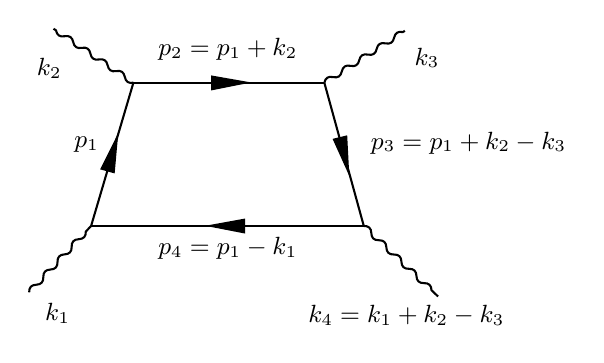
\begin{tikzpicture}[x=0.75pt,y=0.75pt,yscale=-1,xscale=1]
%uncomment if require: \path (0,300); %set diagram left start at 0, and has height of 300

%Straight Lines [id:da9043496640872404] 
\draw    (441.45,125) -- (533.45,125) ;
%Straight Lines [id:da5157434322955703] 
\draw    (421.07,194) -- (552.45,194) ;
%Straight Lines [id:da785623349636802] 
\draw    (533.45,125) -- (552.45,194) ;
%Straight Lines [id:da2309448833125134] 
\draw    (441.45,125) -- (421.07,194) ;
%Straight Lines [id:da7081283804373899] 
\draw    (441.45,125) .. controls (439.14,125.45) and (437.76,124.51) .. (437.31,122.2) .. controls (436.86,119.89) and (435.48,118.95) .. (433.17,119.4) .. controls (430.86,119.85) and (429.47,118.91) .. (429.02,116.6) .. controls (428.57,114.29) and (427.19,113.35) .. (424.88,113.8) .. controls (422.57,114.25) and (421.19,113.31) .. (420.74,111) .. controls (420.29,108.69) and (418.91,107.75) .. (416.6,108.2) .. controls (414.29,108.65) and (412.9,107.71) .. (412.45,105.4) .. controls (412,103.09) and (410.62,102.15) .. (408.31,102.6) .. controls (406,103.05) and (404.62,102.11) .. (404.17,99.8) -- (402.97,98.98) -- (402.97,98.98) ;
%Straight Lines [id:da9717590902584281] 
\draw    (391.23,225.98) .. controls (391.15,223.63) and (392.29,222.41) .. (394.64,222.33) .. controls (396.99,222.24) and (398.13,221.02) .. (398.05,218.67) .. controls (397.97,216.32) and (399.11,215.1) .. (401.46,215.01) .. controls (403.81,214.93) and (404.95,213.71) .. (404.88,211.36) .. controls (404.8,209.01) and (405.94,207.79) .. (408.29,207.7) .. controls (410.64,207.62) and (411.78,206.4) .. (411.7,204.05) .. controls (411.62,201.7) and (412.76,200.48) .. (415.11,200.39) .. controls (417.46,200.3) and (418.6,199.08) .. (418.52,196.73) -- (421.07,194) -- (421.07,194) ;
%Straight Lines [id:da16119065445107128] 
\draw    (533.45,125) .. controls (533.94,122.69) and (535.34,121.79) .. (537.65,122.29) .. controls (539.96,122.79) and (541.36,121.89) .. (541.85,119.58) .. controls (542.35,117.27) and (543.75,116.37) .. (546.06,116.87) .. controls (548.37,117.37) and (549.77,116.47) .. (550.26,114.16) .. controls (550.75,111.85) and (552.15,110.95) .. (554.46,111.45) .. controls (556.77,111.95) and (558.17,111.05) .. (558.66,108.74) .. controls (559.15,106.43) and (560.55,105.53) .. (562.86,106.03) .. controls (565.17,106.53) and (566.57,105.63) .. (567.06,103.32) .. controls (567.56,101.01) and (568.96,100.11) .. (571.27,100.61) -- (572.23,99.98) -- (572.23,99.98) ;
%Straight Lines [id:da2458087873096113] 
\draw    (552.45,194) .. controls (554.8,193.94) and (556.01,195.09) .. (556.08,197.44) .. controls (556.14,199.79) and (557.35,200.94) .. (559.7,200.89) .. controls (562.05,200.83) and (563.26,201.98) .. (563.33,204.33) .. controls (563.39,206.68) and (564.6,207.83) .. (566.95,207.77) .. controls (569.31,207.71) and (570.52,208.86) .. (570.58,211.22) .. controls (570.64,213.57) and (571.85,214.72) .. (574.2,214.66) .. controls (576.55,214.6) and (577.76,215.75) .. (577.83,218.1) .. controls (577.89,220.45) and (579.1,221.6) .. (581.45,221.55) .. controls (583.8,221.49) and (585.01,222.64) .. (585.08,224.99) -- (588.23,227.98) -- (588.23,227.98) ;
%Shape: Triangle [id:dp17567016354284792] 
\draw  [fill={rgb, 255:red, 0; green, 0; blue, 0 }  ,fill opacity=1 ] (495.49,124.91) -- (479.44,128.11) -- (479.38,122.07) -- cycle ;
%Shape: Triangle [id:dp9679845903221488] 
\draw  [fill={rgb, 255:red, 0; green, 0; blue, 0 }  ,fill opacity=1 ] (544.84,167.31) -- (538.12,152.4) -- (543.99,150.97) -- cycle ;
%Shape: Triangle [id:dp021727061775353662] 
\draw  [fill={rgb, 255:red, 0; green, 0; blue, 0 }  ,fill opacity=1 ] (478.72,193.95) -- (494.82,191.03) -- (494.78,197.07) -- cycle ;
%Shape: Triangle [id:dp7820952252000707] 
\draw  [fill={rgb, 255:red, 0; green, 0; blue, 0 }  ,fill opacity=1 ] (433.44,151.76) -- (431.98,168.06) -- (426.16,166.42) -- cycle ;

% Text Node
\draw (400.95,118) node  [font=\small]  {$k_{2}$};
% Text Node
\draw (404.95,236) node  [font=\small]  {$k_{1}$};
% Text Node
\draw (572.95,237) node  [font=\small]  {$k_{4} =k_{1} +k_{2} -k_{3}$};
% Text Node
\draw (582.95,113) node  [font=\small]  {$k_{3}$};
% Text Node
\draw (418.95,155) node  [font=\small]  {$p_{1}$};
% Text Node
\draw (486.95,109) node  [font=\small]  {$p_{2} =p_{1} +k_{2}$};
% Text Node
\draw (486.95,205) node  [font=\small]  {$p_{4} =p_{1} -k_{1}$};
% Text Node
\draw (602.95,154) node  [font=\small]  {$p_{3} =p_{1} +k_{2} -k_{3}$};


\end{tikzpicture}

    \caption{One way for Photon-photon scattering}
    \label{fig:photon-photon-scattering}
\end{figure}
Using Feynman rules, the second order amplitude for the photon-photon scattering of Fig. (\ref{fig:photon-photon-scattering}), where we distinguish that diagram from its sibling diagrams with the subscript (a), is
$$M_{(a)}=\varepsilon_{\mu}\left(\mathbf{k}_{4}\right) \varepsilon_{v}\left(\mathbf{k}_{3}\right) \varepsilon_{\rho}\left(\mathbf{k}_{2}\right) \varepsilon_{\sigma}\left(\mathbf{k}_{1}\right) \times$$
$$\underbrace{\frac{-e_{0}^{4}}{(2 \pi)^{4}} \operatorname{Tr} \int \frac{1}{\not p_{4}-m+i \varepsilon} \gamma^{\mu} \frac{1}{\not p_{3}-m+i \varepsilon} \gamma^{\nu} \frac{1}{\not p_{2}-m+i \varepsilon} \gamma^{\rho} \frac{1}{\not p_{1}-m+i \varepsilon} \gamma^{\sigma} d^{4} p_{1}}_{\mathcal{M}^{\mu\nu\rho\sigma}_{(a)}}$$
From our Ward identities ( \ref{ward-identity-2} ), where letter subscripts represent different sub-amplitudes contributing to the total second order amplitude, we have
$$k_{1 \mu} \mathcal{M}_{\gamma\gamma \rightarrow \gamma\gamma}^{\mu v o \sigma}=0$$
For $k_{1 \mu}$ being arbitrary (any possible components), this can only be true if $\mathcal{M}^{\mu\nu\rho\sigma}_{\gamma\gamma \rightarrow \gamma\gamma}$ is finite. Therefore, \textbf{the amplitude for light-light scattering does not diverge.}
\begin{qt}
    Each of the following being true implies the others are also.
    \begin{easylist}
    \NewList
    @ The theory is locally gauge invariant(locally symmetric)
    @ A quantity (charge) is conserved
    @ The theory has the correct interactions
    @ The Ward identities hold
    @ The theory is renormalizable
    \end{easylist}
    If the above are true, then \textbf{the gauge boson(photon) is massless.}
\end{qt}

\section{Changes in the Theory with \texorpdfstring{$m$ instead of $m_0$}{TEXT}}
\subsection{Counterterms in Lagrangian and Hamiltonian}
If we need to use the measured mass $m$, we need to investigate what that means for the QED Lagrangian
$$\mathcal{L}=-\frac{1}{4} F^{\mu v} F_{\mu v}+\bar{\psi}\left(i \gamma^{\mu} \partial_{\mu}-m_{0}\right) \psi+e_{0} \bar{\psi} \gamma^{\mu} \psi A_{\mu}$$
We can get the Lagrangian into a form with $m$ by substituting $m_{0}=m-\dot{c} m$
\begin{equation}\mathcal{L}=-\frac{1}{4} F^{\mu v} F_{\mu v}+\bar{\psi}\left(i \gamma^{\mu} \partial_{\mu}-m\right) \psi+\underbrace{e_{0} \bar{\psi} \gamma^{\mu} \psi A_{\mu}+\overbrace{\delta m \bar{\psi} \psi}^{\text{mass counter term}}}_{\text{mass normalized }\mathcal{L}_I}
\end{equation}
Recall that $\mathcal{L}_{I}=-\mathcal{H}_{I}$ and that \textbf{each term in $\mathcal{L}_{I}$ (or equivalently, $\mathcal{H}_{l}$ ) represents an interaction} (a vertex, typically, in the sense that it gives rise to a corresponding vertex in a Feynman diagram).

\redp{If we want to use a Lagrangian with the measured mass instead of the bare mass, We must also include a fermion self-interaction diagram} as shown in the RHS of Fig.(\ref{fig:free-fermion-self-interaction}):
\begin{figure}[H]
    \centering
\tikzset{every picture/.style={line width=0.75pt}} %set default line width to 0.75pt        

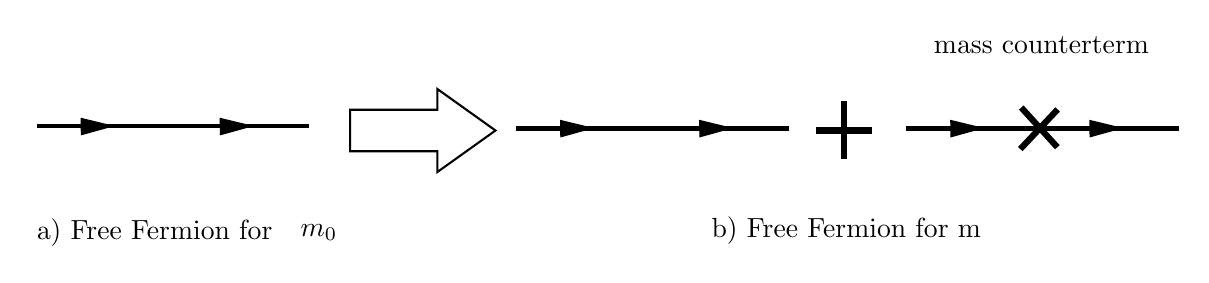
\begin{tikzpicture}[x=0.75pt,y=0.75pt,yscale=-1,xscale=1]
%uncomment if require: \path (0,180); %set diagram left start at 0, and has height of 180

%Straight Lines [id:da9310282435163652] 
\draw [line width=1.5]    (47,87) -- (178.25,87) ;
%Shape: Triangle [id:dp4548894723713879] 
\draw  [fill={rgb, 255:red, 0; green, 0; blue, 0 }  ,fill opacity=1 ] (149.6,86.86) -- (135.71,90.72) -- (135.59,83.47) -- cycle ;
%Shape: Triangle [id:dp7513325146028341] 
\draw  [fill={rgb, 255:red, 0; green, 0; blue, 0 }  ,fill opacity=1 ] (82.6,86.86) -- (68.71,90.72) -- (68.59,83.47) -- cycle ;
%Straight Lines [id:da6718752695134704] 
\draw [line width=1.5]    (278,88) -- (409.25,88) ;
%Shape: Triangle [id:dp7724736634484227] 
\draw  [fill={rgb, 255:red, 0; green, 0; blue, 0 }  ,fill opacity=1 ] (380.6,87.86) -- (366.71,91.72) -- (366.59,84.47) -- cycle ;
%Shape: Triangle [id:dp35362607852135675] 
\draw  [fill={rgb, 255:red, 0; green, 0; blue, 0 }  ,fill opacity=1 ] (313.6,87.86) -- (299.71,91.72) -- (299.59,84.47) -- cycle ;
%Straight Lines [id:da1386824218582332] 
\draw [line width=1.5]    (466,88) -- (597.25,88) ;
%Shape: Triangle [id:dp048955239277462925] 
\draw  [fill={rgb, 255:red, 0; green, 0; blue, 0 }  ,fill opacity=1 ] (568.6,87.86) -- (554.71,91.72) -- (554.59,84.47) -- cycle ;
%Shape: Triangle [id:dp4053274966798466] 
\draw  [fill={rgb, 255:red, 0; green, 0; blue, 0 }  ,fill opacity=1 ] (501.6,87.86) -- (487.71,91.72) -- (487.59,84.47) -- cycle ;
%Straight Lines [id:da031036743918025578] 
\draw [line width=2.25]    (521.33,77.95) -- (538.71,97.06) ;
%Straight Lines [id:da28067901345752844] 
\draw [line width=2.25]    (538.85,78.84) -- (520.85,97.95) ;
%Straight Lines [id:da4376314317638925] 
\draw [line width=2.25]    (436.03,74.95) -- (436.03,102.95) ;
%Straight Lines [id:da9940284951946451] 
\draw [line width=2.25]    (449.55,88.95) -- (422.5,88.95) ;
%Right Arrow [id:dp6053188228931834] 
\draw   (198,79) -- (240,79) -- (240,69) -- (268,89) -- (240,109) -- (240,99) -- (198,99) -- cycle ;

% Text Node
\draw (533.27,48) node   [align=left] {
mass counterterm
};
% Text Node
\draw (437,137) node   [align=left] {b) Free Fermion for m};
% Text Node
\draw (106,138) node   [align=left] {a) Free Fermion for };
% Text Node
\draw (183,138) node    {$m_{0}$};


\end{tikzpicture}
    \caption{Equivalent Free Fermion Feynman Diagrams}
    \label{fig:free-fermion-self-interaction}
\end{figure}
Thus, \textbf{our Feynman rule for this term is}
\begin{qt}
    10. For each mass counterterm diagram, add a term to the Feynman amplitude with a factor equal to $i\delta m$.
\end{qt}
With mass renormalized, the Dirac equation is
\begin{equation}\left(i \gamma^{\alpha} \partial_{\alpha}-m\right) \psi=0\end{equation}

\section{\texorpdfstring{B in $\Pi(p)$ = L in $\Lambda^{\mu}(p,p^{\prime})$}{TEXT}}

 Let's now express $\Lambda^{\mu}\left(p, p^{\prime}\right)$ in its most general possible form. \bluep{Such a form must contain all possible related entities in the theory having components $\mu$, and these are simply $\gamma^{\mu}$,$p^{\mu}$, and $p^{\prime\mu}$.} Thus,
 \begin{equation}
 \Lambda^{\mu}\left(p, p^{\prime}\right)=a \gamma^{\mu}+b_{1} p^{\mu}+b_{2} p^{\prime \mu}
 \label{general-Lambda}
 \end{equation}
 $\Lambda^{\mu}\left(p, p^{\prime}\right)$ represents a vertex. If $p=p^{\prime}$, then \textbf{$\Lambda^{\mu}\left(p, p)\right)$ represent a free fermion with the vertex loop becoming a fermion self-energy loop.}
 
 Thus, where $p=p^{\prime}$ and $b=b_{1}+b_{2}$, (\ref{general-Lambda}) becomes
 $$\Lambda^{\mu}(p, p)=a \gamma^{\mu}+b p^{\mu} \rightarrow \bar{u}_{r}(\mathbf{p}) \Lambda^{\mu}(p, p) u_{r}(\mathbf{p})=\bar{u}_{r}(\mathbf{p}) a \gamma^{\mu} u_{r}(\mathbf{p})+\bar{u}_{r}(\mathbf{p}) b p^{\mu} u_{r}(\mathbf{p})$$
 
 In Gordon's identity (\ref{gordon-identity}) that when $p^{\prime}=p$, we have
 $$\bar{u}_{r}(\mathbf{p}) \gamma^{\mu} u_{r}(\mathbf{p})=\frac{p^{\mu}+p^{\mu}}{2 m} \bar{u}_{r}(\mathbf{p}) u_{r}(\mathbf{p})=\frac{p^{\mu}}{m} \bar{u}_{r}(\mathbf{p}) u_{r}(\mathbf{p})$$
 and
 $$
 \bar{u}_{r}(\mathbf{p}) \Lambda^{\mu}(p, p) u_{r}(\mathbf{p})=a \bar{u}_{r}(\mathbf{p}) \gamma^{\mu} u_{r}(\mathbf{p})+m b \bar{u}_{r}(\mathbf{p}) \gamma^{\mu} u_{r}(\mathbf{p})
 $$
 So,
 $$\bar{u}_{r}(\mathbf{p}) \Lambda^{\mu}(p, p) u_{r}(\mathbf{p})=L \bar{u}_{r}(\mathbf{p}) \gamma^{\mu} u_{r}(\mathbf{p}) \quad \text { where } L=a+m b$$
 Thus,$\Lambda^{\mu}(p, p)=L(\Lambda) \gamma^{\mu}$, and
 
 $$\Lambda^{\mu}\left(p, p^{\prime}\right)=\underbrace{L(\Lambda) \gamma^{\mu}}_{\text{free particle part}}+\underbrace{\Lambda_{c}^{\mu}\left(p, p^{\prime}\right)}_{=0,for(p=p')}$$
 From the original Ward identity,
 $$\bar{u}_{r}(\mathbf{p}) \frac{\partial \Sigma(p)}{\partial p_{\mu}} u_{r}(\mathbf{p})=\bar{u}_{r}(\mathbf{p}) \Lambda^{\mu}(p, p) u_{r}(\mathbf{p})$$
 $$=\bar{u}_{r}(\mathbf{p}) \frac{\partial}{\partial p_{\mu}}\left(A+\left(p_{v} \gamma^{v}-m\right) B+\left(p_{v} \gamma^{v}-m\right) \Sigma_{c}\right) u_{r}(\mathbf{p})=\bar{u}_{r}(\mathbf{p}) L \gamma^{\mu} u_{r}(\mathbf{p})$$
 $$=\bar{u}_{r}(\mathbf{p}) \gamma^{\mu} B u_{r}(\mathbf{p})+\bar{u}_{r}(\mathbf{p}) \gamma^{\mu} \underbrace{\Sigma_{c}\left(\not p-m\right) u_{r}(\mathbf{p})}_{=0}+\underbrace{\overline{u_{r}}(\mathbf{p})(\not p-m)}_{=0} \frac{\partial}{\partial p_{\mu}} \Sigma_{c}(\not p-m) u_{r}(\mathbf{p})
 $$
 Note that $\Sigma_{c}(\not p-m)$ is part of an expansion in $p-m,$ so each term in it has $\not p-m$ raised to a power. The factor of $\cancel{p}-m$ on the right in any such term acts on $u_r(\mathbf{p})$ results in zero. Thus,
 \begin{equation}B \bar{u}_{r}(\mathbf{p}) \gamma^{\mu} u_{r}(\mathbf{p})=L \bar{u}_{r}(\mathbf{p}) \gamma^{\mu} u_{r}(\mathbf{p}) \rightarrow B=L\end{equation}
 
 \section{Re-expressing 2nd Order Corrections}
 \subsection{The 2nd Order Photon Propagator}
 The figure below shows how the \textbf{Feynman diagram for the photon propagator at first order becomes two diagrams at second order.}
 \begin{figure}[H]
     \centering
\tikzset{every picture/.style={line width=0.75pt}} %set default line width to 0.75pt        

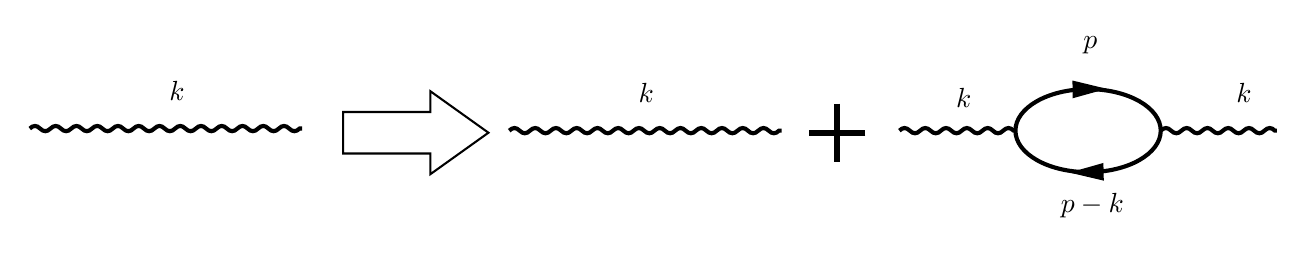
\begin{tikzpicture}[x=0.75pt,y=0.75pt,yscale=-1,xscale=1]
%uncomment if require: \path (0,180); %set diagram left start at 0, and has height of 180

%Straight Lines [id:da9310282435163652] 
\draw [line width=1.5]    (47,87) .. controls (48.67,85.33) and (50.33,85.33) .. (52,87) .. controls (53.67,88.67) and (55.33,88.67) .. (57,87) .. controls (58.67,85.33) and (60.33,85.33) .. (62,87) .. controls (63.67,88.67) and (65.33,88.67) .. (67,87) .. controls (68.67,85.33) and (70.33,85.33) .. (72,87) .. controls (73.67,88.67) and (75.33,88.67) .. (77,87) .. controls (78.67,85.33) and (80.33,85.33) .. (82,87) .. controls (83.67,88.67) and (85.33,88.67) .. (87,87) .. controls (88.67,85.33) and (90.33,85.33) .. (92,87) .. controls (93.67,88.67) and (95.33,88.67) .. (97,87) .. controls (98.67,85.33) and (100.33,85.33) .. (102,87) .. controls (103.67,88.67) and (105.33,88.67) .. (107,87) .. controls (108.67,85.33) and (110.33,85.33) .. (112,87) .. controls (113.67,88.67) and (115.33,88.67) .. (117,87) .. controls (118.67,85.33) and (120.33,85.33) .. (122,87) .. controls (123.67,88.67) and (125.33,88.67) .. (127,87) .. controls (128.67,85.33) and (130.33,85.33) .. (132,87) .. controls (133.67,88.67) and (135.33,88.67) .. (137,87) .. controls (138.67,85.33) and (140.33,85.33) .. (142,87) .. controls (143.67,88.67) and (145.33,88.67) .. (147,87) .. controls (148.67,85.33) and (150.33,85.33) .. (152,87) .. controls (153.67,88.67) and (155.33,88.67) .. (157,87) .. controls (158.67,85.33) and (160.33,85.33) .. (162,87) .. controls (163.67,88.67) and (165.33,88.67) .. (167,87) .. controls (168.67,85.33) and (170.33,85.33) .. (172,87) .. controls (173.67,88.67) and (175.33,88.67) .. (177,87) -- (178.25,87) -- (178.25,87) ;
%Straight Lines [id:da6718752695134704] 
\draw [line width=1.5]    (278,88) .. controls (279.67,86.33) and (281.33,86.33) .. (283,88) .. controls (284.67,89.67) and (286.33,89.67) .. (288,88) .. controls (289.67,86.33) and (291.33,86.33) .. (293,88) .. controls (294.67,89.67) and (296.33,89.67) .. (298,88) .. controls (299.67,86.33) and (301.33,86.33) .. (303,88) .. controls (304.67,89.67) and (306.33,89.67) .. (308,88) .. controls (309.67,86.33) and (311.33,86.33) .. (313,88) .. controls (314.67,89.67) and (316.33,89.67) .. (318,88) .. controls (319.67,86.33) and (321.33,86.33) .. (323,88) .. controls (324.67,89.67) and (326.33,89.67) .. (328,88) .. controls (329.67,86.33) and (331.33,86.33) .. (333,88) .. controls (334.67,89.67) and (336.33,89.67) .. (338,88) .. controls (339.67,86.33) and (341.33,86.33) .. (343,88) .. controls (344.67,89.67) and (346.33,89.67) .. (348,88) .. controls (349.67,86.33) and (351.33,86.33) .. (353,88) .. controls (354.67,89.67) and (356.33,89.67) .. (358,88) .. controls (359.67,86.33) and (361.33,86.33) .. (363,88) .. controls (364.67,89.67) and (366.33,89.67) .. (368,88) .. controls (369.67,86.33) and (371.33,86.33) .. (373,88) .. controls (374.67,89.67) and (376.33,89.67) .. (378,88) .. controls (379.67,86.33) and (381.33,86.33) .. (383,88) .. controls (384.67,89.67) and (386.33,89.67) .. (388,88) .. controls (389.67,86.33) and (391.33,86.33) .. (393,88) .. controls (394.67,89.67) and (396.33,89.67) .. (398,88) .. controls (399.67,86.33) and (401.33,86.33) .. (403,88) .. controls (404.67,89.67) and (406.33,89.67) .. (408,88) -- (409.25,88) -- (409.25,88) ;
%Straight Lines [id:da1386824218582332] 
\draw [line width=1.5]    (466,88) .. controls (467.67,86.33) and (469.33,86.33) .. (471,88) .. controls (472.67,89.67) and (474.33,89.67) .. (476,88) .. controls (477.67,86.33) and (479.33,86.33) .. (481,88) .. controls (482.67,89.67) and (484.33,89.67) .. (486,88) .. controls (487.67,86.33) and (489.33,86.33) .. (491,88) .. controls (492.67,89.67) and (494.33,89.67) .. (496,88) .. controls (497.67,86.33) and (499.33,86.33) .. (501,88) .. controls (502.67,89.67) and (504.33,89.67) .. (506,88) .. controls (507.67,86.33) and (509.33,86.33) .. (511,88) .. controls (512.67,89.67) and (514.33,89.67) .. (516,88) .. controls (517.67,86.33) and (519.33,86.33) .. (521,88) -- (521.9,88) -- (521.9,88) ;
%Shape: Triangle [id:dp048955239277462925] 
\draw  [fill={rgb, 255:red, 0; green, 0; blue, 0 }  ,fill opacity=1 ] (563.87,67.88) -- (549.99,71.74) -- (549.87,64.49) -- cycle ;
%Straight Lines [id:da4376314317638925] 
\draw [line width=2.25]    (436.03,74.95) -- (436.03,102.95) ;
%Straight Lines [id:da9940284951946451] 
\draw [line width=2.25]    (449.55,88.95) -- (422.5,88.95) ;
%Right Arrow [id:dp6053188228931834] 
\draw   (198,79) -- (240,79) -- (240,69) -- (268,89) -- (240,109) -- (240,99) -- (198,99) -- cycle ;
%Shape: Ellipse [id:dp9485847747999785] 
\draw  [line width=1.5]  (521.9,88) .. controls (521.9,76.95) and (537.57,68) .. (556.9,68) .. controls (576.23,68) and (591.9,76.95) .. (591.9,88) .. controls (591.9,99.05) and (576.23,108) .. (556.9,108) .. controls (537.57,108) and (521.9,99.05) .. (521.9,88) -- cycle ;
%Shape: Triangle [id:dp6030894239400264] 
\draw  [fill={rgb, 255:red, 0; green, 0; blue, 0 }  ,fill opacity=1 ] (549.93,108.16) -- (563.79,104.22) -- (563.96,111.46) -- cycle ;
%Straight Lines [id:da6021332528094747] 
\draw [line width=1.5]    (591.9,88) .. controls (593.57,86.33) and (595.23,86.33) .. (596.9,88) .. controls (598.57,89.67) and (600.23,89.67) .. (601.9,88) .. controls (603.57,86.33) and (605.23,86.33) .. (606.9,88) .. controls (608.57,89.67) and (610.23,89.67) .. (611.9,88) .. controls (613.57,86.33) and (615.23,86.33) .. (616.9,88) .. controls (618.57,89.67) and (620.23,89.67) .. (621.9,88) .. controls (623.57,86.33) and (625.23,86.33) .. (626.9,88) .. controls (628.57,89.67) and (630.23,89.67) .. (631.9,88) .. controls (633.57,86.33) and (635.23,86.33) .. (636.9,88) .. controls (638.57,89.67) and (640.23,89.67) .. (641.9,88) .. controls (643.57,86.33) and (645.23,86.33) .. (646.9,88) -- (647.8,88) -- (647.8,88) ;

% Text Node
\draw (118,69) node    {$k$};
% Text Node
\draw (344,70) node    {$k$};
% Text Node
\draw (497,72) node    {$k$};
% Text Node
\draw (632,70) node    {$k$};
% Text Node
\draw (558,47) node    {$p$};
% Text Node
\draw (559,124) node    {$p-k$};


\end{tikzpicture}

     \caption{Photon Propagator Self-energy Correction to 2nd Order in $\alpha$}
     \label{fig:2nd-order-photon-propagator}
 \end{figure}
 
 This means the photon propagator becomes
 \begin{equation}i D_{F \alpha \beta}(k) \Rightarrow i D_{F \alpha \beta}^{2 n d}=i D_{F \alpha \beta}(k)+i D_{F \alpha \mu}(k) i e_{0}^{2} \Pi^{\mu \nu}(k) i D_{F \nu \beta}(k)
 \label{2nd-photon-propagator}
 \end{equation}
 The RHS of (\ref{2nd-photon-propagator}) is thus
 $$i D_{F \alpha \beta}^{2 n d}(k)=-\frac{i g_{a \beta}}{k^{2}+i \varepsilon}+\frac{-i g_{\alpha \mu}}{k^{2}+i \varepsilon} i e_{0}^{2} g^{\mu \nu}\left(-k^{2} A^{\prime}(k, \Lambda)-k^{2} \Pi_{c}\left(k^{2}\right)\right)\underbrace{\frac{-i g_{v \beta}}{k^{2}+i \varepsilon}}_{\approx k^{2}}$$
 $$=\frac{-i g_{\alpha \beta}}{k^{2}+i \varepsilon}+\frac{-i g_{\alpha \mu}}{k^{2}+i \varepsilon} e_{0}^{2} \delta^{\mu}{}_\beta\left(-A^{\prime}(k, \Lambda)-\Pi_{c}\left(k^{2}\right)\right)=\underbrace{\frac{-i g_{\alpha \beta}}{k^{2}+i \varepsilon}}_{iD_{F\alpha\beta}(k)}\left(1-e_{0}^{2} A^{\prime}(k, \Lambda)-e_{0}^{2} \Pi_{c}\left(k^{2}\right)\right)
 $$
 So
 \begin{qt}
     \begin{equation}
         iD_{F\alpha\beta}^{2nd}(k)=iD_{F\alpha\beta}\left(1-e_{0}^{2} A^{\prime}(k, \Lambda)-e_{0}^{2} \Pi_{c}\left(k^{2}\right)\right)
     \end{equation}
 \end{qt}
 
 \subsection{The 2nd Order Fermion Propagator}
 The figure below depicts Feynman diagrams for two different ways we can represent the 2nd order fermion propagator, depending on whether we wish to work with $m_0$ or $m$.
 \begin{figure}[H]
     \centering
\tikzset{every picture/.style={line width=0.75pt}} %set default line width to 0.75pt        

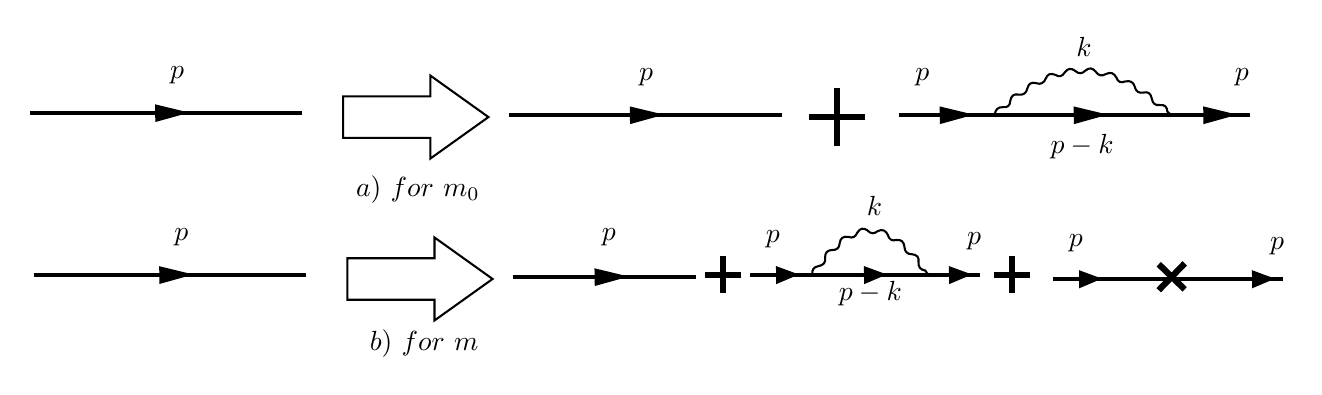
\begin{tikzpicture}[x=0.75pt,y=0.75pt,yscale=-1,xscale=1]
%uncomment if require: \path (0,180); %set diagram left start at 0, and has height of 180

%Straight Lines [id:da9310282435163652] 
\draw [line width=1.5]    (28,44) -- (159.25,44) ;
%Straight Lines [id:da6718752695134704] 
\draw [line width=1.5]    (259,45) -- (390.25,45) ;
%Straight Lines [id:da1386824218582332] 
\draw [line width=1.5]    (447,45) -- (615.97,45) ;
%Shape: Triangle [id:dp048955239277462925] 
\draw  [fill={rgb, 255:red, 0; green, 0; blue, 0 }  ,fill opacity=1 ] (607.87,44.88) -- (593.99,48.74) -- (593.87,41.49) -- cycle ;
%Straight Lines [id:da4376314317638925] 
\draw [line width=2.25]    (417.03,31.95) -- (417.03,59.95) ;
%Straight Lines [id:da9940284951946451] 
\draw [line width=2.25]    (430.55,45.95) -- (403.5,45.95) ;
%Right Arrow [id:dp6053188228931834] 
\draw   (179,36) -- (221,36) -- (221,26) -- (249,46) -- (221,66) -- (221,56) -- (179,56) -- cycle ;
%Shape: Triangle [id:dp45244019773334176] 
\draw  [fill={rgb, 255:red, 0; green, 0; blue, 0 }  ,fill opacity=1 ] (102.87,43.88) -- (88.99,47.74) -- (88.87,40.49) -- cycle ;
%Shape: Triangle [id:dp6891242809250332] 
\draw  [fill={rgb, 255:red, 0; green, 0; blue, 0 }  ,fill opacity=1 ] (331.6,44.88) -- (317.71,48.74) -- (317.59,41.49) -- cycle ;
%Shape: Triangle [id:dp29069725308704386] 
\draw  [fill={rgb, 255:red, 0; green, 0; blue, 0 }  ,fill opacity=1 ] (480.87,44.88) -- (466.99,48.74) -- (466.87,41.49) -- cycle ;
%Shape: Triangle [id:dp7015070240747568] 
\draw  [fill={rgb, 255:red, 0; green, 0; blue, 0 }  ,fill opacity=1 ] (545.46,44.88) -- (531.57,48.74) -- (531.45,41.49) -- cycle ;
%Curve Lines [id:da9505483667309718] 
\draw    (492.87,44.95) .. controls (493.23,42.32) and (494.57,41.07) .. (496.89,41.22) .. controls (499.15,41.46) and (500.32,40.45) .. (500.41,38.2) .. controls (500.85,35.73) and (502.16,34.71) .. (504.34,35.15) .. controls (506.72,35.5) and (508.15,34.51) .. (508.64,32.19) .. controls (509.21,29.88) and (510.63,29.03) .. (512.89,29.66) .. controls (515.04,30.43) and (516.59,29.67) .. (517.53,27.4) .. controls (518.33,25.27) and (519.86,24.69) .. (522.13,25.66) .. controls (523.95,26.85) and (525.47,26.45) .. (526.69,24.44) .. controls (528.1,22.5) and (529.76,22.26) .. (531.65,23.71) .. controls (533.34,25.29) and (534.99,25.26) .. (536.6,23.61) .. controls (538.42,22.06) and (540.07,22.23) .. (541.56,24.11) .. controls (542.85,26.06) and (544.5,26.43) .. (546.53,25.23) .. controls (548.74,24.18) and (550.4,24.75) .. (551.53,26.95) .. controls (552.24,29.06) and (553.64,29.7) .. (555.73,28.85) .. controls (558.23,28.28) and (559.78,29.14) .. (560.39,31.41) .. controls (560.91,33.7) and (562.34,34.63) .. (564.67,34.18) .. controls (566.8,33.65) and (568.1,34.6) .. (568.57,37.03) .. controls (568.98,39.47) and (570.3,40.53) .. (572.52,40.2) .. controls (574.79,39.96) and (575.98,40.99) .. (576.07,43.3) -- (577.87,44.95) ;
%Straight Lines [id:da5710561468306551] 
\draw [line width=1.5]    (30,122) -- (161.25,122) ;
%Straight Lines [id:da0006488658837261463] 
\draw [line width=1.5]    (261,123) -- (349.23,123) ;
%Straight Lines [id:da25376426972818955] 
\draw [line width=1.5]    (375,122) -- (485.87,122) ;
%Shape: Triangle [id:dp15882997893103257] 
\draw  [fill={rgb, 255:red, 0; green, 0; blue, 0 }  ,fill opacity=1 ] (480.56,121.88) -- (471.44,125.74) -- (471.36,118.49) -- cycle ;
%Straight Lines [id:da9198596278195672] 
\draw [line width=2.25]    (362.19,112.95) -- (362.19,130.95) ;
%Straight Lines [id:da06447104513693658] 
\draw [line width=2.25]    (370.89,121.95) -- (353.5,121.95) ;
%Right Arrow [id:dp0683396683347155] 
\draw   (181,114) -- (223,114) -- (223,104) -- (251,124) -- (223,144) -- (223,134) -- (181,134) -- cycle ;
%Shape: Triangle [id:dp4259767598404586] 
\draw  [fill={rgb, 255:red, 0; green, 0; blue, 0 }  ,fill opacity=1 ] (104.87,121.88) -- (90.99,125.74) -- (90.87,118.49) -- cycle ;
%Shape: Triangle [id:dp4223432398676771] 
\draw  [fill={rgb, 255:red, 0; green, 0; blue, 0 }  ,fill opacity=1 ] (314.6,122.88) -- (300.71,126.74) -- (300.59,119.49) -- cycle ;
%Shape: Triangle [id:dp04700781442223034] 
\draw  [fill={rgb, 255:red, 0; green, 0; blue, 0 }  ,fill opacity=1 ] (397.23,121.88) -- (388.11,125.74) -- (388.03,118.49) -- cycle ;
%Shape: Triangle [id:dp7554295771540895] 
\draw  [fill={rgb, 255:red, 0; green, 0; blue, 0 }  ,fill opacity=1 ] (439.6,121.88) -- (430.49,125.74) -- (430.41,118.49) -- cycle ;
%Curve Lines [id:da5856879781635035] 
\draw    (405.1,121.95) .. controls (404.72,119.57) and (405.69,118.19) .. (408.02,117.82) .. controls (410.49,117.35) and (411.54,116.01) .. (411.19,113.8) .. controls (411.1,111.37) and (412.23,110.12) .. (414.6,110.03) .. controls (416.86,110.15) and (418.07,109.03) .. (418.24,106.66) .. controls (418.55,104.31) and (419.93,103.32) .. (422.38,103.7) .. controls (424.39,104.5) and (425.85,103.81) .. (426.75,101.62) .. controls (428.04,99.53) and (429.66,99.2) .. (431.63,100.61) .. controls (433.12,102.28) and (434.75,102.41) .. (436.5,100.98) .. controls (438.69,99.88) and (440.33,100.46) .. (441.4,102.73) .. controls (441.99,104.96) and (443.36,105.8) .. (445.51,105.23) .. controls (447.86,104.94) and (449.15,106) .. (449.4,108.41) .. controls (449.52,110.85) and (450.74,112.08) .. (453.06,112.09) .. controls (455.47,112.3) and (456.51,113.52) .. (456.2,115.75) .. controls (456.03,118.23) and (457.1,119.61) .. (459.4,119.9) -- (460.87,121.95) ;
%Straight Lines [id:da8454096833616818] 
\draw [line width=1.5]    (521,124) -- (631.87,124) ;
%Shape: Triangle [id:dp7831515590478635] 
\draw  [fill={rgb, 255:red, 0; green, 0; blue, 0 }  ,fill opacity=1 ] (626.56,123.88) -- (617.44,127.74) -- (617.36,120.49) -- cycle ;
%Shape: Triangle [id:dp3712751967961748] 
\draw  [fill={rgb, 255:red, 0; green, 0; blue, 0 }  ,fill opacity=1 ] (543.23,123.88) -- (534.11,127.74) -- (534.03,120.49) -- cycle ;
%Straight Lines [id:da04439645146016946] 
\draw [line width=2.25]    (501.19,112.95) -- (501.19,130.95) ;
%Straight Lines [id:da14678419627563355] 
\draw [line width=2.25]    (509.89,121.95) -- (492.5,121.95) ;
%Straight Lines [id:da25279856519358535] 
\draw [line width=2.25]    (584.46,116.48) -- (571.93,129.42) ;
%Straight Lines [id:da61960383144899] 
\draw [line width=2.25]    (584.44,129) -- (571.95,116.9) ;

% Text Node
\draw (99,26) node    {$p$};
% Text Node
\draw (325,27) node    {$p$};
% Text Node
\draw (458,27) node    {$p$};
% Text Node
\draw (536,12) node    {$k$};
% Text Node
\draw (535,60) node    {$p-k$};
% Text Node
\draw (612,27) node    {$p$};
% Text Node
\draw (101,104) node    {$p$};
% Text Node
\draw (307,104) node    {$p$};
% Text Node
\draw (386,105) node    {$p$};
% Text Node
\draw (435,89) node    {$k$};
% Text Node
\draw (433,131) node    {$p-k$};
% Text Node
\draw (483,106) node    {$p$};
% Text Node
\draw (532,107) node    {$p$};
% Text Node
\draw (629,108) node    {$p$};
% Text Node
\draw (215,81) node    {$a) \ for\ m_{0}$};
% Text Node
\draw (218,155) node    {$b) \ for\ m$};


\end{tikzpicture}
     \caption{Fermion Propagator Self-energy Correction to Diagrams of 2nd Order in $\alpha$}
     \label{fig:2nd-fermion-propagator}
 \end{figure}
 We will work with a) here first. Thus, the 2nd order fermion propagator is
 \begin{equation}i S_{F}(p) \Rightarrow i S_{F}^{2 n d}(p)=i S_{F}(p)+i S_{F}(p) i e_{0}^{2} \Sigma(p) i S_{F}(p)\end{equation}
 and 
 $$i S_{F}^{2 n d}(p)=i \frac{1}{\underbrace{\cancel{p}-m_{0}+i \varepsilon}_{A \text { operator }}}+\underbrace{i \frac{1}{\cancel{p}-m_{0}+i \varepsilon}}_{A \text { operator }} \underbrace{\left(-e_{0}^{2} \Sigma(p)\right)}_{B \text { operator }}\frac{1}{\not p-m_{0}+i \varepsilon}$$
 $$=\frac{i}{A-B}+\left(\begin{array}{l}
\text { higher } \\
\text { order }
\end{array}\right)$$
$$=\frac{i}{\not p\underbrace{-m_{0}+e_{0}^{2} A(\Lambda, m)}_{-m}+e_{0}^{2}(\not p-m) B(\Lambda)+e_{0}^{2}(\not p-m) \Sigma_{c}(\not p-m)+i \varepsilon}+h.o.$$
where $A(\Lambda, m)$ is unbounded, actually $A(\Lambda, m) \rightarrow-\infty$. And h.o. means higher order corrections. Thus, our renormalized fermion propagator to 2nd order, is
$$
i S_{F}^{2 n d}(p)=\frac{i\left(1+e_{0}^{2} B(\Lambda)+e_{0}^{2} \Sigma_{c}(\not p-m)\right)^{-1}}{(\cancel{p}-m)+i \varepsilon\left(1+e_{0}^{2} B(\Lambda)+e_{0}^{2} \Sigma_{c}(\not p-m)\right)^{-1}}+h.o.
$$
$$
=\frac{i\left(1+e_{0}^{2} B(\Lambda)+e_{0}^{2} \Sigma_{c}(\not p-m)\right)^{-1}}{(\not p-m)+i \varepsilon\left(1+e_{0}^{2} B(\Lambda)+e_{0}^{2} \Sigma_{c}(\not p-m)\right)^{-1}}+h.o.
$$
Using $\frac{1}{1+x}=1-x+\ldots$, we have
$$
iS_{F}^{2nd}(p)=\frac{i\left(1-e_{0}^{2} B(\Lambda)-e_{0}^{2} \Sigma_{c}(\not p-m)\right)}{(\not p-m)+i \varepsilon\left(1-e_{0}^{2} B(\Lambda)-e_{0}^{2} \Sigma_{c}(\not p-m)\right)}+h.o.$$
$$=\underbrace{\frac{i}{\not p-m+i \varepsilon}}_{i S_{F}(p)}\left(1-e_{0}^{2} B(\Lambda)-e_{0}^{2} \Sigma_{c}(\not p-m)\right)+h.o.$$
So
\begin{qt}
    \begin{equation}
        iS_{F}^{2nd}(p)\approx i S_{F}(p)\left(1-e_{0}^{2} B(\Lambda)-e_{0}^{2} \Sigma_{c}(\not p-m)\right)
    \end{equation}
\end{qt}

\subsection{2nd Order Incoming and Outgoing Particles}
We also have to include higher order corrections to the incoming and outgoing particles, not just the propagators and vertices. The external 2nd fermion corrections, for example, is depicted below
\begin{figure}[H]
    \centering

\tikzset{every picture/.style={line width=0.75pt}} %set default line width to 0.75pt        

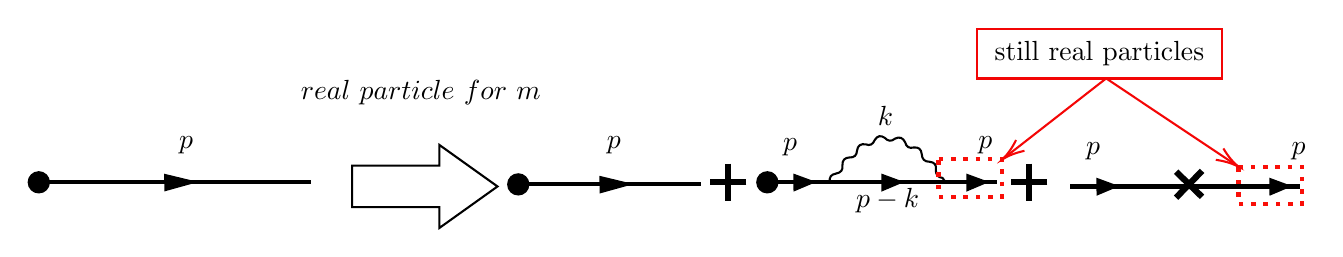
\begin{tikzpicture}[x=0.75pt,y=0.75pt,yscale=-1,xscale=1]
%uncomment if require: \path (0,180); %set diagram left start at 0, and has height of 180

%Straight Lines [id:da5710561468306551] 
\draw [line width=1.5]    (24,122) -- (155.25,122) ;
\draw [shift={(24,122)}, rotate = 0] [color={rgb, 255:red, 0; green, 0; blue, 0 }  ][fill={rgb, 255:red, 0; green, 0; blue, 0 }  ][line width=1.5]      (0, 0) circle [x radius= 4.36, y radius= 4.36]   ;
%Straight Lines [id:da0006488658837261463] 
\draw [line width=1.5]    (255,123) -- (343.23,123) ;
\draw [shift={(255,123)}, rotate = 0] [color={rgb, 255:red, 0; green, 0; blue, 0 }  ][fill={rgb, 255:red, 0; green, 0; blue, 0 }  ][line width=1.5]      (0, 0) circle [x radius= 4.36, y radius= 4.36]   ;
%Straight Lines [id:da25376426972818955] 
\draw [line width=1.5]    (375,122) -- (485.87,122) ;
\draw [shift={(375,122)}, rotate = 0] [color={rgb, 255:red, 0; green, 0; blue, 0 }  ][fill={rgb, 255:red, 0; green, 0; blue, 0 }  ][line width=1.5]      (0, 0) circle [x radius= 4.36, y radius= 4.36]   ;
%Shape: Triangle [id:dp15882997893103257] 
\draw  [fill={rgb, 255:red, 0; green, 0; blue, 0 }  ,fill opacity=1 ] (480.56,121.88) -- (471.44,125.74) -- (471.36,118.49) -- cycle ;
%Straight Lines [id:da9198596278195672] 
\draw [line width=2.25]    (356.19,112.95) -- (356.19,130.95) ;
%Straight Lines [id:da06447104513693658] 
\draw [line width=2.25]    (364.89,121.95) -- (347.5,121.95) ;
%Right Arrow [id:dp0683396683347155] 
\draw   (175,114) -- (217,114) -- (217,104) -- (245,124) -- (217,144) -- (217,134) -- (175,134) -- cycle ;
%Shape: Triangle [id:dp4259767598404586] 
\draw  [fill={rgb, 255:red, 0; green, 0; blue, 0 }  ,fill opacity=1 ] (98.87,121.88) -- (84.99,125.74) -- (84.87,118.49) -- cycle ;
%Shape: Triangle [id:dp4223432398676771] 
\draw  [fill={rgb, 255:red, 0; green, 0; blue, 0 }  ,fill opacity=1 ] (308.6,122.88) -- (294.71,126.74) -- (294.59,119.49) -- cycle ;
%Shape: Triangle [id:dp04700781442223034] 
\draw  [fill={rgb, 255:red, 0; green, 0; blue, 0 }  ,fill opacity=1 ] (397.23,121.88) -- (388.11,125.74) -- (388.03,118.49) -- cycle ;
%Shape: Triangle [id:dp7554295771540895] 
\draw  [fill={rgb, 255:red, 0; green, 0; blue, 0 }  ,fill opacity=1 ] (439.6,121.88) -- (430.49,125.74) -- (430.41,118.49) -- cycle ;
%Curve Lines [id:da5856879781635035] 
\draw    (405.1,121.95) .. controls (404.72,119.57) and (405.69,118.19) .. (408.02,117.82) .. controls (410.49,117.35) and (411.54,116.01) .. (411.19,113.8) .. controls (411.1,111.37) and (412.23,110.12) .. (414.6,110.03) .. controls (416.86,110.15) and (418.07,109.03) .. (418.24,106.66) .. controls (418.55,104.31) and (419.93,103.32) .. (422.38,103.7) .. controls (424.39,104.5) and (425.85,103.81) .. (426.75,101.62) .. controls (428.04,99.53) and (429.66,99.2) .. (431.63,100.61) .. controls (433.12,102.28) and (434.75,102.41) .. (436.5,100.98) .. controls (438.69,99.88) and (440.33,100.46) .. (441.4,102.73) .. controls (441.99,104.96) and (443.36,105.8) .. (445.51,105.23) .. controls (447.86,104.94) and (449.15,106) .. (449.4,108.41) .. controls (449.52,110.85) and (450.74,112.08) .. (453.06,112.09) .. controls (455.47,112.3) and (456.51,113.52) .. (456.2,115.75) .. controls (456.03,118.23) and (457.1,119.61) .. (459.4,119.9) -- (460.87,121.95) ;
%Straight Lines [id:da8454096833616818] 
\draw [line width=1.5]    (521,124) -- (631.87,124) ;
%Shape: Triangle [id:dp7831515590478635] 
\draw  [fill={rgb, 255:red, 0; green, 0; blue, 0 }  ,fill opacity=1 ] (626.56,123.88) -- (617.44,127.74) -- (617.36,120.49) -- cycle ;
%Shape: Triangle [id:dp3712751967961748] 
\draw  [fill={rgb, 255:red, 0; green, 0; blue, 0 }  ,fill opacity=1 ] (543.23,123.88) -- (534.11,127.74) -- (534.03,120.49) -- cycle ;
%Straight Lines [id:da04439645146016946] 
\draw [line width=2.25]    (501.19,112.95) -- (501.19,130.95) ;
%Straight Lines [id:da14678419627563355] 
\draw [line width=2.25]    (509.89,121.95) -- (492.5,121.95) ;
%Straight Lines [id:da25279856519358535] 
\draw [line width=2.25]    (584.46,116.48) -- (571.93,129.42) ;
%Straight Lines [id:da61960383144899] 
\draw [line width=2.25]    (584.44,129) -- (571.95,116.9) ;
%Shape: Rectangle [id:dp04478205879951447] 
\draw  [color={rgb, 255:red, 249; green, 15; blue, 8 }  ,draw opacity=1 ][dash pattern={on 1.69pt off 2.76pt}][line width=1.5]  (457.5,110.95) -- (488.25,110.95) -- (488.25,128.95) -- (457.5,128.95) -- cycle ;
%Shape: Rectangle [id:dp7516437787148507] 
\draw  [color={rgb, 255:red, 249; green, 15; blue, 8 }  ,draw opacity=1 ][dash pattern={on 1.69pt off 2.76pt}][line width=1.5]  (601.99,114.49) -- (632.74,114.49) -- (632.74,132.49) -- (601.99,132.49) -- cycle ;
%Straight Lines [id:da8146287403873916] 
\draw [color={rgb, 255:red, 244; green, 6; blue, 6 }  ,draw opacity=1 ]   (538.25,71.95) -- (489.83,109.72) ;
\draw [shift={(488.25,110.95)}, rotate = 322.05] [color={rgb, 255:red, 244; green, 6; blue, 6 }  ,draw opacity=1 ][line width=0.75]    (10.93,-3.29) .. controls (6.95,-1.4) and (3.31,-0.3) .. (0,0) .. controls (3.31,0.3) and (6.95,1.4) .. (10.93,3.29)   ;
%Straight Lines [id:da4262402767955018] 
\draw [color={rgb, 255:red, 244; green, 6; blue, 6 }  ,draw opacity=1 ]   (538.25,71.95) -- (600.33,113.38) ;
\draw [shift={(601.99,114.49)}, rotate = 213.72] [color={rgb, 255:red, 244; green, 6; blue, 6 }  ,draw opacity=1 ][line width=0.75]    (10.93,-3.29) .. controls (6.95,-1.4) and (3.31,-0.3) .. (0,0) .. controls (3.31,0.3) and (6.95,1.4) .. (10.93,3.29)   ;

% Text Node
\draw (95,104) node    {$p$};
% Text Node
\draw (301,104) node    {$p$};
% Text Node
\draw (386,105) node    {$p$};
% Text Node
\draw (433,131) node    {$p-k$};
% Text Node
\draw (480,104) node    {$p$};
% Text Node
\draw (532,107) node    {$p$};
% Text Node
\draw (631,107) node    {$p$};
% Text Node
\draw (208,79) node    {$real\ particle\ for\ m$};
% Text Node
\draw (432,90) node    {$k$};
% Text Node
\draw  [color={rgb, 255:red, 242; green, 5; blue, 5 }  ,draw opacity=1 ]  (476,48) -- (594,48) -- (594,72) -- (476,72) -- cycle  ;
\draw (535,60) node   [align=left] {still real particles};


\end{tikzpicture}

    \caption{Real Fermion Self-energy Correction to Diagrams of 2nd Order in $\alpha$}
    \label{fig:2nd-external-fermion}
\end{figure}
The initial fermion contribution to the amplitude, upon renormalization, becomes (where we note that in the last two diagrams of Fig. (\ref{fig:2nd-external-fermion}) the last line is really an internal line in the overall Feynman diagram for an entire reaction, so must be represented by a propagator)
$$u_{r}(\mathbf{p}) \Rightarrow u_{r}^{2 n d}(\mathbf{p})=u_{r}(\mathbf{p})+\frac{i}{\cancel{p}-m+i \varepsilon} i e_{0}^{2} \Sigma(p) u_{r}(\mathbf{p})+\frac{i}{\cancel{p}-m+i \varepsilon}(i \delta m) u_{r}(\mathbf{p})$$
$$
=\left(1-\frac{e_{0}^{2} A(\Lambda, m)+e_{0}^{2}(\not p-m) B(\Lambda)+e_{0}^{2}(\not p-m) \Sigma_{c}(\not p-m)+\delta m}{\not p-m+i \varepsilon}\right)u_r(\mathbf{p})
$$
since $\delta m=-e_{0}^{2} A(\Lambda, m),$ two terms will cancel above. Also, $e_{0}^{2} \Sigma_{c}(\not p-m)$ is an expansion having terms of $(\not p-m)$ to various powers. So each of these terms will lead to a factor of $(\cancel{p}-m) u_{r}(\mathbf{p})$ above. Thus, 
\begin{equation}u_{r}(\mathbf{p}) \Rightarrow\left(1-\frac{e_{0}^{2}(\not p-m) B(\Lambda)}{\not p-m+i \varepsilon}\right) u_{r}(\mathbf{p}) \quad \text { indeterminate and naive }
\label{naive-2nd-external-fermion}
\end{equation}
We must be wary with (\ref{naive-2nd-external-fermion}) for two reasons. First the \textbf{fermion is real and on shell}, so we might at first consider that $(\not p-m) u_{r}(\mathbf{p})=0$. However, we also have a factor of $\not p-m$ in the denominator, which would make us think the second term would be $e_0^2B(\Lambda)$. We thus do not know really what that second term is.

Second, we have not considered that the incoming fermion is initially bare, but becomes dressed via self-interactions. That is, \textbf{we would need to incorporate the adiabatic hypothesis, whereby $\mathcal{H}_{1}$ is turned off initially, but then is turned on well before the particle begins to interact with any other particle.}

Note that 
$$i S_{F \alpha \beta}(x-y)=\left\langle 0\left|T\left\{\psi_{\alpha}(x) \bar{\psi}_{\beta}(y)\right\}\right| 0\right\rangle$$
where the amplitude has a spinor factor associated with each field. In essence, for the fermion (not anti-fermion) propagator, there is a factor of $u_{r}(\mathbf{p}) \bar{u}_{r}(\mathbf{p})$. To renormalize the propagator, we multiply it by $1-e_{0}^{2} B(\Lambda)-e_{0}^{2} \Sigma_{c}(\not p-m)$. \textbf{\redp{So, in effect, each of the two spinors $u_r$ and $\bar{u}_r$ is multiplied by the square root of $1-e_{0}^{2} B(\Lambda)-e_{0}^{2} \Sigma_{c}(\not p-m)$}}. So we can surmise that the real particle renormalization is the square root of $1-e_{0}^{2} B(\Lambda)-e_{0}^{2} \Sigma_{c}(\not p-m)$, where we drop the $\Sigma_c$ term. This lead to
\begin{qt}
    \begin{equation}\begin{aligned}
&\bar{u}_{r}(\mathbf{p}) \Rightarrow \bar{u}_{r}^{2 n d}(\mathbf{p}) \approx\left(1-\frac{1}{2} e_{0}^{2} B(\Lambda)\right) \bar{u}_{r}(\mathbf{p})\\
&v_{r}(\mathbf{p}) \Rightarrow v_{r}^{2 n d}(\mathbf{p}) \approx\left(1-\frac{1}{2} e_{0}^{2} B(\Lambda)\right) v_{r}(\mathbf{p})\\
&\bar{v}_{r}(\mathbf{p}) \Rightarrow \bar{v}_{r}^{2 n d}(\mathbf{p}) \approx\left(1-\frac{1}{2} e_{0}^{2} B(\Lambda)\right) \bar{v}_{r}(\mathbf{p})\\
&\varepsilon_{\mu}(\mathbf{k}) \Rightarrow \varepsilon_{\mu}^{2 n d}(\mathbf{k}) \approx\left(1-\frac{1}{2} e_{0}^{2} A^{\prime}(\Lambda)\right) \varepsilon_{\mu}(\mathbf{k})
\end{aligned}\end{equation}
\end{qt}
Relations above are often called \textbf{external line renormalizations}

\subsection{The 2nd Order Vetex}
The vertex modification to second order is depicted in the figure below.
\begin{figure}
    \centering
    


\tikzset{every picture/.style={line width=0.75pt}} %set default line width to 0.75pt        

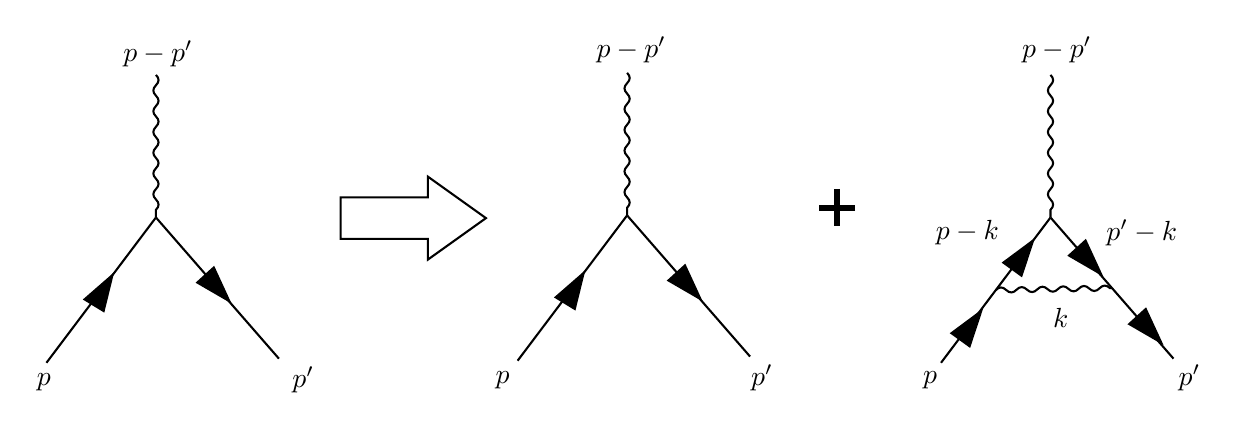
\begin{tikzpicture}[x=0.75pt,y=0.75pt,yscale=-1,xscale=1]
%uncomment if require: \path (0,276); %set diagram left start at 0, and has height of 276

%Straight Lines [id:da5443514830848077] 
\draw    (102,58) .. controls (103.67,59.67) and (103.67,61.33) .. (102,63) .. controls (100.33,64.67) and (100.33,66.33) .. (102,68) .. controls (103.67,69.67) and (103.67,71.33) .. (102,73) .. controls (100.33,74.67) and (100.33,76.33) .. (102,78) .. controls (103.67,79.67) and (103.67,81.33) .. (102,83) .. controls (100.33,84.67) and (100.33,86.33) .. (102,88) .. controls (103.67,89.67) and (103.67,91.33) .. (102,93) .. controls (100.33,94.67) and (100.33,96.33) .. (102,98) .. controls (103.67,99.67) and (103.67,101.33) .. (102,103) .. controls (100.33,104.67) and (100.33,106.33) .. (102,108) .. controls (103.67,109.67) and (103.67,111.33) .. (102,113) .. controls (100.33,114.67) and (100.33,116.33) .. (102,118) .. controls (103.67,119.67) and (103.67,121.33) .. (102,123) -- (102,126.7) -- (102,126.7) ;
%Straight Lines [id:da4951270349524055] 
\draw    (102,126.7) -- (161.25,194.7) ;
%Straight Lines [id:da023703889707956782] 
\draw    (102,126.7) -- (49.25,196.7) ;
%Shape: Triangle [id:dp22768971699307095] 
\draw  [fill={rgb, 255:red, 0; green, 0; blue, 0 }  ,fill opacity=1 ] (81.05,154.44) -- (76.79,171.76) -- (67.6,166.15) -- cycle ;
%Shape: Triangle [id:dp07516182653589565] 
\draw  [fill={rgb, 255:red, 0; green, 0; blue, 0 }  ,fill opacity=1 ] (137.35,166.99) -- (121.92,158.04) -- (129.88,150.79) -- cycle ;
%Right Arrow [id:dp24961982071595235] 
\draw   (191,117) -- (233,117) -- (233,107) -- (261,127) -- (233,147) -- (233,137) -- (191,137) -- cycle ;
%Straight Lines [id:da4753078406756951] 
\draw    (329,57) .. controls (330.67,58.67) and (330.67,60.33) .. (329,62) .. controls (327.33,63.67) and (327.33,65.33) .. (329,67) .. controls (330.67,68.67) and (330.67,70.33) .. (329,72) .. controls (327.33,73.67) and (327.33,75.33) .. (329,77) .. controls (330.67,78.67) and (330.67,80.33) .. (329,82) .. controls (327.33,83.67) and (327.33,85.33) .. (329,87) .. controls (330.67,88.67) and (330.67,90.33) .. (329,92) .. controls (327.33,93.67) and (327.33,95.33) .. (329,97) .. controls (330.67,98.67) and (330.67,100.33) .. (329,102) .. controls (327.33,103.67) and (327.33,105.33) .. (329,107) .. controls (330.67,108.67) and (330.67,110.33) .. (329,112) .. controls (327.33,113.67) and (327.33,115.33) .. (329,117) .. controls (330.67,118.67) and (330.67,120.33) .. (329,122) -- (329,125.7) -- (329,125.7) ;
%Straight Lines [id:da651626427422886] 
\draw    (329,125.7) -- (388.25,193.7) ;
%Straight Lines [id:da34490859808991636] 
\draw    (329,125.7) -- (276.25,195.7) ;
%Shape: Triangle [id:dp8427547117716038] 
\draw  [fill={rgb, 255:red, 0; green, 0; blue, 0 }  ,fill opacity=1 ] (308.05,153.44) -- (303.79,170.76) -- (294.6,165.15) -- cycle ;
%Shape: Triangle [id:dp5478379509434596] 
\draw  [fill={rgb, 255:red, 0; green, 0; blue, 0 }  ,fill opacity=1 ] (364.35,165.99) -- (348.92,157.04) -- (356.88,149.79) -- cycle ;
%Straight Lines [id:da8662809658931607] 
\draw [line width=2.25]    (430.19,112.95) -- (430.19,130.95) ;
%Straight Lines [id:da5465002539608441] 
\draw [line width=2.25]    (438.89,121.95) -- (421.5,121.95) ;
%Straight Lines [id:da9756118391117254] 
\draw    (533,58) .. controls (534.67,59.67) and (534.67,61.33) .. (533,63) .. controls (531.33,64.67) and (531.33,66.33) .. (533,68) .. controls (534.67,69.67) and (534.67,71.33) .. (533,73) .. controls (531.33,74.67) and (531.33,76.33) .. (533,78) .. controls (534.67,79.67) and (534.67,81.33) .. (533,83) .. controls (531.33,84.67) and (531.33,86.33) .. (533,88) .. controls (534.67,89.67) and (534.67,91.33) .. (533,93) .. controls (531.33,94.67) and (531.33,96.33) .. (533,98) .. controls (534.67,99.67) and (534.67,101.33) .. (533,103) .. controls (531.33,104.67) and (531.33,106.33) .. (533,108) .. controls (534.67,109.67) and (534.67,111.33) .. (533,113) .. controls (531.33,114.67) and (531.33,116.33) .. (533,118) .. controls (534.67,119.67) and (534.67,121.33) .. (533,123) -- (533,126.7) -- (533,126.7) ;
%Straight Lines [id:da1851162855408226] 
\draw    (533,126.7) -- (592.25,194.7) ;
%Straight Lines [id:da4919051338870595] 
\draw    (533,126.7) -- (480.25,196.7) ;
%Shape: Triangle [id:dp39199193569785507] 
\draw  [fill={rgb, 255:red, 0; green, 0; blue, 0 }  ,fill opacity=1 ] (524.6,137.81) -- (519.01,154.74) -- (510.29,148.44) -- cycle ;
%Shape: Triangle [id:dp5651924374997691] 
\draw  [fill={rgb, 255:red, 0; green, 0; blue, 0 }  ,fill opacity=1 ] (557.35,153.99) -- (541.92,145.04) -- (549.88,137.79) -- cycle ;
%Shape: Triangle [id:dp9516288946136692] 
\draw  [fill={rgb, 255:red, 0; green, 0; blue, 0 }  ,fill opacity=1 ] (499.6,171.81) -- (494.01,188.74) -- (485.29,182.44) -- cycle ;
%Shape: Triangle [id:dp25021011569224283] 
\draw  [fill={rgb, 255:red, 0; green, 0; blue, 0 }  ,fill opacity=1 ] (586.35,186.99) -- (570.92,178.04) -- (578.88,170.79) -- cycle ;
%Straight Lines [id:da09690258041950939] 
\draw    (506.63,161.7) .. controls (508.26,160.01) and (509.93,159.98) .. (511.62,161.61) .. controls (513.31,163.24) and (514.98,163.21) .. (516.62,161.52) .. controls (518.26,159.83) and (519.93,159.8) .. (521.62,161.43) .. controls (523.31,163.06) and (524.98,163.03) .. (526.62,161.34) .. controls (528.26,159.65) and (529.93,159.62) .. (531.62,161.25) .. controls (533.31,162.88) and (534.98,162.85) .. (536.62,161.16) .. controls (538.26,159.47) and (539.93,159.44) .. (541.62,161.08) .. controls (543.31,162.71) and (544.98,162.68) .. (546.62,160.99) .. controls (548.26,159.3) and (549.93,159.27) .. (551.62,160.9) .. controls (553.31,162.53) and (554.98,162.5) .. (556.62,160.81) .. controls (558.26,159.12) and (559.93,159.09) .. (561.62,160.72) -- (562.63,160.7) -- (562.63,160.7) ;

% Text Node
\draw (538,175) node    {$k$};
% Text Node
\draw (475,205) node    {$p$};
% Text Node
\draw (600,204) node    {$p^{\prime }$};
% Text Node
\draw (536,46) node    {$p-p^{\prime }$};
% Text Node
\draw (577,134) node    {$p^{\prime } -k$};
% Text Node
\draw (493,134) node    {$p -k$};
% Text Node
\draw (331,46) node    {$p-p^{\prime }$};
% Text Node
\draw (269,205) node    {$p$};
% Text Node
\draw (394,204) node    {$p^{\prime }$};
% Text Node
\draw (48,206) node    {$p$};
% Text Node
\draw (173,205) node    {$p^{\prime }$};
% Text Node
\draw (103,48) node    {$p-p^{\prime }$};


\end{tikzpicture}

    \caption{Vertex Correction to 2nd Order in $\alpha$}
    \label{fig:2nd-vertex}
\end{figure}
$$i_{0_{0} \gamma}^{\mu} \Rightarrow i e_{0} \gamma_{2 n d}^{\mu}\left(p, p^{\prime}\right)=i e_{0}\left(\gamma^{\mu}-\left(i e_{0}\right)^{2} \Lambda^{\mu}\left(p, p^{\prime}\right)\right)$$
and
\begin{qt}
    \begin{equation}i e_{0} \gamma^{\mu} \Rightarrow i e_{0} \gamma_{2 n d}^{\mu}\left(p, p^{\prime}\right)=i e_{0}\left\{\gamma^{\mu}\left(1+e_{0}^{2} L(\Lambda)\right)+e_{0}^{2} \Lambda_{c}^{\mu}\left(p, p^{\prime}\right)\right\}
    \label{2nd-vertex}
    \end{equation}
\end{qt}